\chapter{Construction d'un document {\LaTeX}}
\label{chap:construction}


\begin{conseil}
  Utilisez impérativement les commandes {\LaTeX} pour identifier
  les différentes parties (la structure) d'un document.
\end{conseil}

\section{Structure logique d'un livre}

(classes \class{book}, \class{memoir}, \class{ulthese})

\begin{lstlisting}
\frontmatter
\end{lstlisting}
\begin{itemize}
\item préface, table des matières, etc.
\item numérotation des pages en chiffres romains (i, ii, ...)
\item chapitres non numérotés
\end{itemize}

\begin{lstlisting}
\mainmatter
\end{lstlisting}
\begin{itemize}
\item le contenu à proprement parler
\item numérotation des pages à partir de 1 en chiffres arabes
\item chapitres numérotés
\end{itemize}

\begin{lstlisting}
\backmatter
\end{lstlisting}
\begin{itemize}
\item tout le reste (bibliographie, index, etc.)
\item numérotation des pages se poursuit
\item chapitres non numérotés
\end{itemize}


\section{Titre et page titre}

\begin{itemize}
\item Mise en forme automatique
\begin{lstlisting}
%% préambule
\title`\marg{Titre du document}'
\author`\marg{Prénom Nom}'
\date`\marg{1{\ier} janvier 1970}' % automatique si omis

%% corps du document
\maketitle
\end{lstlisting}
\item Mise en forme libre
  \begin{minipage}{0.45\linewidth}
    classes standards
\begin{lstlisting}
\begin{titlepage}
  ...
\end{titlepage}
\end{lstlisting}
  \end{minipage}
  \hfill
  \begin{minipage}{0.45\linewidth}
    classe \class{memoir}
\begin{lstlisting}
\begin{titlingpage}
  ...
\end{titlingpage}
\end{lstlisting}
  \end{minipage}
\end{itemize}

\section{Résumé}

\begin{itemize}
\item Classes \class{article}, \class{report} ou \class{memoir}:
  résumé créé avec l'environnement
\begin{lstlisting}
\begin{abstract}

\end{abstract}
\end{lstlisting}
\item Classe \class{ulthese}: résumés français et anglais traités
  comme des chapitres normaux (non numérotés).
\end{itemize}


\section{Table des matières}

\begin{itemize}
\item Table des matières produite automatiquement avec
\begin{lstlisting}
\tableofcontents
\end{lstlisting}
\item Requiert plusieurs compilations
\item Sections non numérotées pas incluses
\item Avec \pkg{hyperref}, produit également la table des matières du
  fichier PDF
\item Classe \class{memoir} fournit également
\begin{lstlisting}
\tableofcontents*
\end{lstlisting}
  qui n'insère pas la table des matières dans la table des matières
\item Aussi disponibles:
\begin{lstlisting}
\listoffigures
\listoftables
\end{lstlisting}
  (et leurs versions \verb=*= dans \class{memoir})
\end{itemize}


\section{Sections}

\begin{itemize}
\item Découpage du document en sections avec les commandes
\begin{lstlisting}
\part`\marg{titre}'
\chapter`\marg{titre}'
\section`\marg{titre}'
\subsection`\marg{titre}'
\subsubsection`\marg{titre}'
\paragraph`\marg{titre}'
\end{lstlisting}
\item Prennent le titre en argument
\item Numérotation automatique
\item Commande suivie d'une \verb=*= = section non numérotée
\item Éviter d'utiliser des sous-sous-sections
  (\cmdprint{\subsubsection}) dans un livre puisque cela résulte en
  une numérotation à quatre niveaux qui s'avère difficile à suivre pour le
  lecteur.
\item Nous n'avons jamais utilisé le niveau de division \cmdprint{\paragraph}.
\end{itemize}


\section{Annexes}

\begin{itemize}
\item Les annexes sont des sections ou des chapitres avec une
  numérotation alphanumérique (A, A.1, ...)
\item Sections suivantes identifiées comme des annexes par la commande
\begin{lstlisting}
\appendix
\end{lstlisting}
\item Dans le titre, «Chapitre» changé pour «Annexe» le cas échéant
\end{itemize}


\section{Renvois automatiques}
\label{sec:construction:renvois}


\subsection{Étiquettes et renvois}

Parce que l'ordinateur le fera mieux que vous

\begin{itemize}
\item Ne \emph{jamais} renvoyer manuellement à un numéro de section,
  d'équation, de tableau, etc.
\item «Nommer» un élément avec \verb=\label=
\item Faire référence par son nom avec \verb=\ref=
\item Requiert 2 à 3 compilations
\end{itemize}

\begin{demo}
\begin{lstlisting}[emph={\label,\ref}]
\section{Définitions}
\label{sec:definitions}

Lorem ipsum dolor sit amet, consectetur
adipiscing elit. Duis in auctor dui. Vestibulum

\section{Historique}

Tel que vu à la section \ref{sec:definitions},
on a...
\end{lstlisting}
  \begin{framed}
    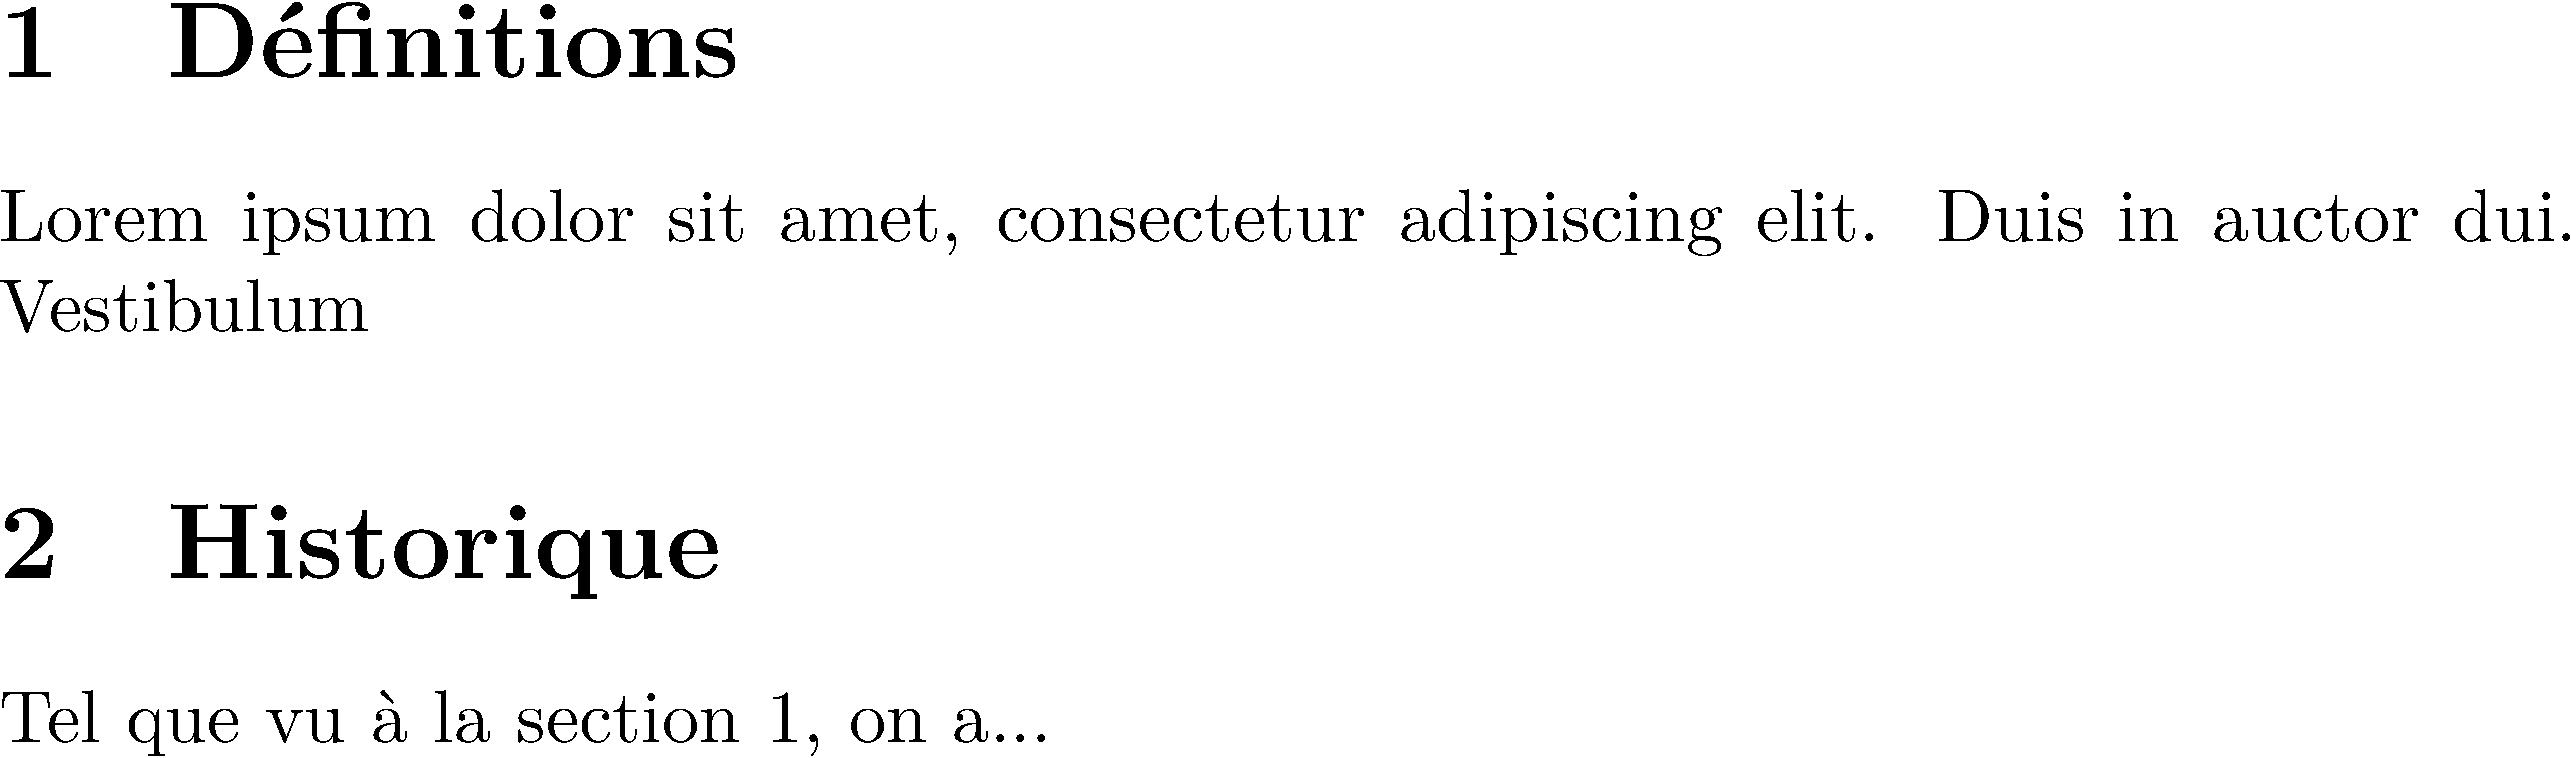
\includegraphics[width=\linewidth]{renvoi}
  \end{framed}
\end{demo}

\begin{conseil}
  Adoptez une manière systématique et mnémotechnique de nommer les
  éléments dans un long document afin de vous y retrouver.

  \bigskip %
  Exemple:
\begin{lstlisting}
\label{chap:`\meta{chapitre}'}          % chapitre
\label{sec:`\meta{chapitre}':`\meta{section}'}  % section
\label{tab:`\meta{chapitre}':`\meta{tableau}'}  % tableau
\label{eq:`\meta{chapitre}':`\meta{equation}'}  % équation
\end{lstlisting}
\end{conseil}


\subsection{Hyperliens}

Renvois automatiques++

\begin{itemize}
\item Paquetage \pkg{hyperref} insère des hyperliens vers les renvois
  dans les fichiers PDF
  \begin{demo}
\begin{lstlisting}
Tel que vu à la section \ref{sec:definitions},
on a...
\end{lstlisting}
    \begin{framed}
      
\includegraphics{renvoi_avec_ref}
    \end{framed}
  \end{demo}
\item Commande \verb=\autoref= permet de
  \begin{enumerate}
  \item nommer automatiquement le type de renvoi (section, équation,
    tableau, etc.)
  \item transformer en hyperlien le texte \textbf{et} le numéro
  \end{enumerate}
  \begin{demo}
\begin{lstlisting}
Tel que vu à la \autoref{sec:definitions},
on a...
\end{lstlisting}
    \begin{framed}
      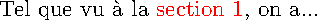
\includegraphics{renvoi_avec_autoref}
    \end{framed}
  \end{demo}
\end{itemize}



%%%
%%% Exercices
%%%

\section{Exercices}
\label{sec:construction:exercices}

\begin{exercice}[nosol]
  Utiliser le fichier \fichier{exercice\_parties.tex}.
  \begin{enumerate}
  \item Étudier la structure du document dans le code source.
  \item Ajouter un titre et un auteur au document.
  \item Créer la table des matières du document en le compilant 2 à 3
    fois.
  \item Insérer deux ou trois titres de sections de différents niveaux
    dans le document.
  \item Vous remarquerez que la numérotation cesse à partir des
    sous-sections. C'est une particularité de la classe
    \class{memoir}.

    Recompiler le document après avoir ajouté au préambule la commande
\begin{lstlisting}
\maxsecnumdepth{subsection}
\end{lstlisting}
  \item Ajouter une annexe au document.
  \end{enumerate}
\end{exercice}

\begin{exercice}[nosol]
  Utiliser le fichier \fichier{exercice\_renvois.tex}.
  \begin{enumerate}
  \item Insérer dans le texte un renvoi au numéro d'une section.
  \item Activer le paquetage \pkg{hyperref} avec l'option
    \code{colorlinks} et comparer l'effet d'utiliser \cmd{\ref} ou
    \cmd{\autoref} pour le renvoi.
  \end{enumerate}
\end{exercice}


%%% Local Variables:
%%% mode: latex
%%% TeX-engine: xetex
%%% TeX-master: "formation_latex_UL-partie_2"
%%% coding: utf-8
%%% End:
